\documentclass{article}
\usepackage{tikz}
\usetikzlibrary{arrows.meta, positioning, calc}
\begin{document}
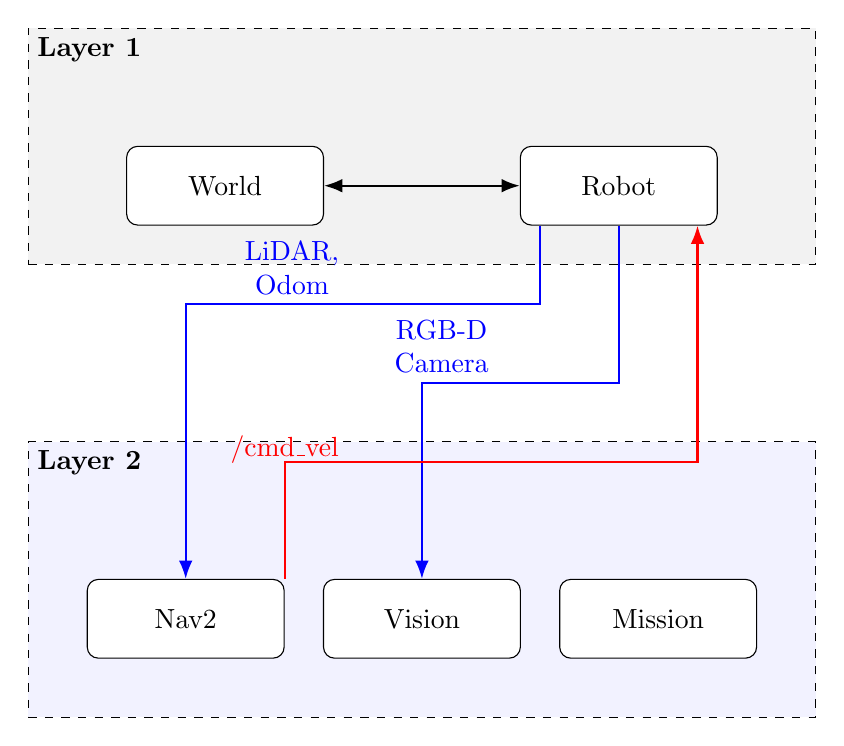
\begin{tikzpicture}[
    box/.style={draw, rectangle, rounded corners, align=center, minimum width=2.5cm, minimum height=1cm},
    >=Latex
]
% Layer 1: Simulation
\node[draw, fill=gray!10, minimum width=10cm, minimum height=3cm, dashed] (layer1) at (0, 0) {};
\node[anchor=north west, font=\bfseries] at (layer1.north west) {Layer 1};
\node[box, fill=white] (world) at (-2.5, -0.5) {World};
\node[box, fill=white] (robot) at (2.5, -0.5) {Robot};
\draw[<->, thick] (world) -- (robot);

% Layer 2: ROS2
\node[draw, fill=blue!5, minimum width=10cm, minimum height=3.5cm, dashed] (layer2) at (0, -5.5) {};
\node[anchor=north west, font=\bfseries] at (layer2.north west) {Layer 2};
\node[box, fill=white] (nav) at (-3, -6) {Nav2};
\node[box, fill=white] (vision) at (0, -6) {Vision};
\node[box, fill=white] (mission) at (3, -6) {Mission};

% Connections
\draw[->, thick, blue] (robot.south) ++(-1,0) -- ++(0,-1) -| node[pos=0.35, above, align=center] {LiDAR,\\Odom} (nav.north);
\draw[->, thick, blue] (robot.south) ++(0,0) -- ++(0,-2) -| node[pos=0.45, above, align=center] {RGB-D\\Camera} (vision.north);
\draw[<-, thick, red] (robot.south) ++(1,0) -- ++(0,-3) -| node[pos=0.55, above] {/cmd\_vel} (nav.north east);

\end{tikzpicture}
\end{document}
